% Appendix A

\chapter{Problemas NP y PH modelados en lógica}
\label{apendiceA}
\lhead{Apéndice A. \emph{Problemas NP y PH modelados en lógica}}

\section{Problemas NP}

\subsection{SAT, Satisfacibilidad proposicional}
\begin{verbatim}
(so-exists (?T 1)
  (forall (?y)
    (exists (?x)
      (or
        (and (?P ?x ?y)
             (?T ?x)) 
        (and (?N ?x ?y)
             (not (?T ?x)))))))
\end{verbatim}

\subsection{CLIQUE, Clique de tamaño $k$}
\begin{verbatim}
(so-exists (?F Inj)
  (and (forall (?y) (exists (?x) (?F ?x ?y)))  ; totality
    (forall (?x) (forall (?y)
      (implies (and (< ?x ?y)
                    (exists (?z) (and (?F ?x ?z) (?K ?z)))
                    (exists (?z) (and (?F ?y ?z) (?K ?z))))
               (?E ?x ?y))))))
\end{verbatim}
\begin{figure}[h!]
\centering
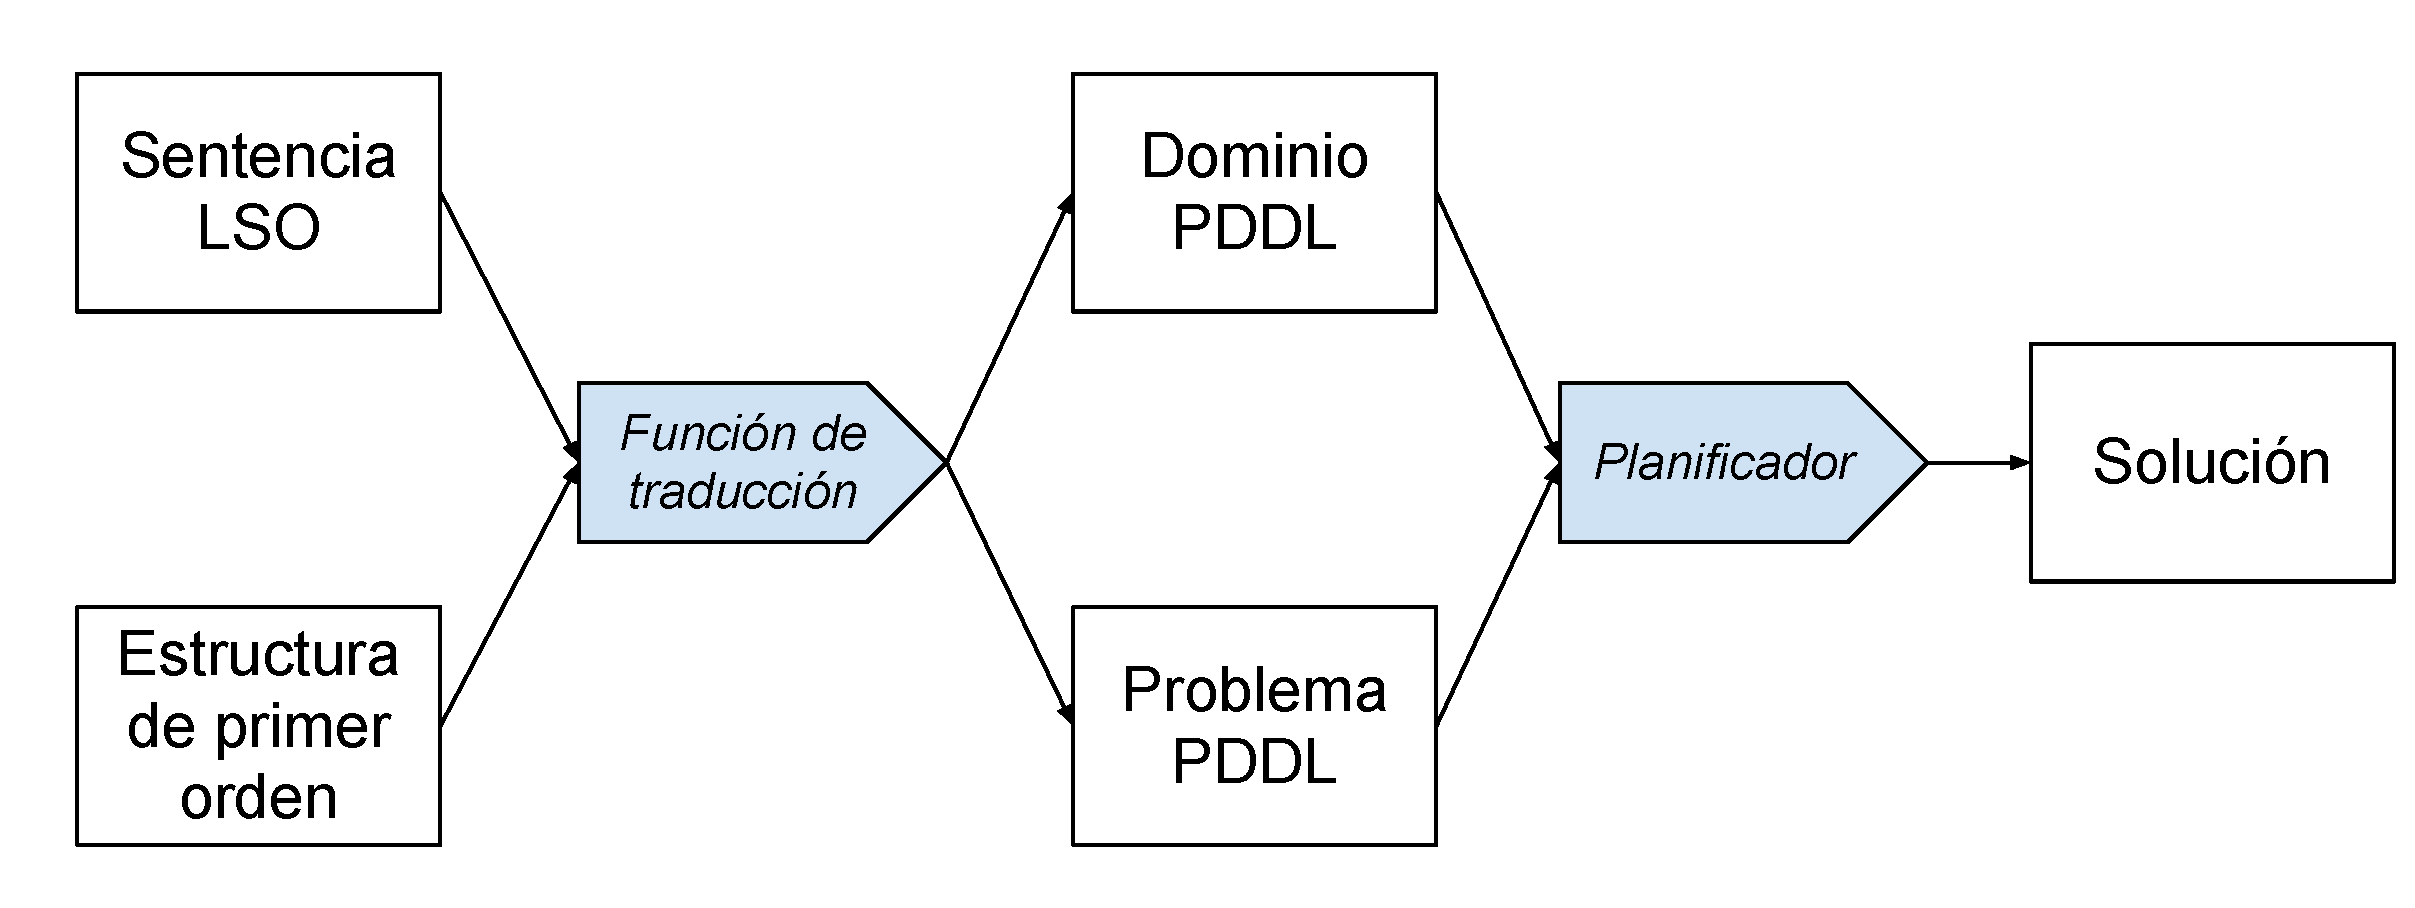
\includegraphics[width=\textwidth]{figuras/esquema_herramienta.pdf}
\caption[Grafo con una \textit{clique} de tamaño $k = 6$]{Grafo con una clique de tamaño
$k = 6$}
\label{clique}
\end{figure}

\begin{verbatim}
(exists F in Inj)(forall x y)[f(x) < K & f(y) < K -> E(x,y)]
\end{verbatim}

\subsection{\CHD, Camino Hamiltoniano Dirigido}
\begin{verbatim}
(so-exists (?F Inj)
  (forall (?x)
    (implies (< ?x MAX)
             (exists (?y1)
               (and (?F ?x ?y1)
                 (exists (?y2)
                   (and
                     (exists (?x2) 
                       (and (SUC ?x ?x2) (?f ?x2 ?y2)))
                   (?E ?y1 ?y2))))))))
\end{verbatim}
\begin{verbatim}
; (exists F in Inj)(forall x)[x < MAX -> E(f(x),f(x+1))]
\end{verbatim}

\subsection{\TDM, \textit{3-Dimensional Matching}}
\begin{verbatim}
(so-exists (?F Inj)
  (so-exists (?G Inj)
    (and
      (forall (?x) (exists (?y) (?F ?x ?y))) ; F is total
      (forall (?x) (exists (?y) (?G ?x ?y))) ; G is total
      (forall (?x) (forall (?y) (forall (?z)
        (implies (and (?F ?x ?y) (?G ?x ?z))
                 (?T ?x ?y ?z))))))))
\end{verbatim}

\subsection{\TCOL, 3-colorabilidad}
\begin{verbatim}
(so-exists (?R 1) (so-exists (?G 1) (so-exists (?B 1)
  (forall (?x) 
    (and
      ; no hay dos vértices adyacentes del mismo color
      (forall (?y)
        (implies (?E ?x ?y) (not (or (and (?R ?x) (?R ?y))
                                        (and (?G ?x) (?G ?y))
                                        (and (?B ?x) (?B ?y))))))

        ; los vértices tienen al menos un color
        (or (?R ?x) (?G ?x) (?B ?x))

        ; los vértices tienen a lo sumo un color
        (implies (?R ?x) (and (not (?G ?x)) (not (?B ?x))))
        (implies (?G ?x) (and (not (?R ?x)) (not (?B ?x))))
        (implies (?B ?x) (and (not (?R ?x)) (not (?G ?x)))))))))
\end{verbatim}

\subsection{\KCOL, k-colorabilidad}
\begin{verbatim}
(so-exists (?F Func)
  (forall (?x) 
    (and (exists (?y) (and (?F ?x ?y) (?K ?y)))
      (forall (?y) 
        (implies (?E ?x ?y)
                 (not (exists (?z)
                   (and (?F ?x ?z) (?F ?y ?z)))))))))
\end{verbatim}

\section{Problemas PH}

\subsection{UNSAT, No-Satisfacibilidad proposicional}
\begin{verbatim}
(so-forall (?T 1 @ist)
    (exists (?y @cls)
        (forall (?x @var)
            (or (and (?N ?x ?y)
                     (?T ?x)
                )
                (and (?P ?x ?y)
                    (not (?T ?x))
                )
                (?NotIn ?x ?y)
             ))))
\end{verbatim}

\subsection{\qEA-QBF, Fórmula \textit{booleana} cuantificada $\Sigma_p^2$}
\begin{verbatim}
(so-exists (?E0 1 @ise0)
    (so-forall (?A0 1 @isa0)
        (forall (?c @cls)
            (exists (?x @var)
                (or
                    (and (?P ?x ?c) (?E0 ?x))
                    (and (?P ?x ?c) (?A0 ?x))
                    (and (?N ?x ?c) (not (?E0 ?x)))
                    (and (?N ?x ?c) (not (?A0 ?x)))
                )))))
\end{verbatim}

\subsection{\coCOL, No-3-Colorabilidad}

\begin{verbatim}
(so-forall (?R 1 @node)
    (so-forall (?G 1 @node)
        (exists (?x @node)
            (or 
                (exists (?y @node)
                    ; no two adjacent vertices of the same color
                    (or (and (?E ?x ?y) (?R ?x) (?R ?y))
                        (and (?E ?x ?y) (?G ?x) (?G ?y))
                        (and (?E ?x ?y) (not (?R ?x)) 
                             (not (?R ?y)) (not (?G ?x)) 
                             (not (?G ?y)))
                    )
                )
                (and (?R ?x) (?G ?x))))))
\end{verbatim}
